\documentclass[a4paper,11pt]{report}

\usepackage{amsmath}
\usepackage{fullpage}
\usepackage{tikz}

\usetikzlibrary{graphs,graphs.standard}

\makeatletter
\pgfmathdeclarefunction{alpha}{1}{%
  \pgfmathint@{#1}%
  \edef\pgfmathresult{\pgffor@alpha{\pgfmathresult}}%
}

\usepackage{bussproofs}
\usepackage{mathpartir}
\usepackage{prooftrees}
\usepackage{color}

\newcommand*{\contract}[2]{contraction of $#1$ with $#2$}

\author{Sylvain Julmy}
\date{\today}

\setlength{\parindent}{0pt}

\begin{document}

\begin{center}
  \Large{
    Mathematical Methods for Computer Science 1\
    Fall 2017
  }
  \noindent\makebox[\linewidth]{\rule{\linewidth}{0.4pt}}

  Series 5
  \vspace*{1.4cm}

  Sylvain Julmy
  
  \noindent\makebox[\linewidth]{\rule{\linewidth}{0.4pt}}
\end{center}

\section*{\texttt{1}}

\subsection*{(a)}
We know that the graph $G=(V,E)$ is $3$-regular. So, $\forall v \in V, deg(v) =
3$. We also know that $\sum_{v \in V} deg(v) = 2|E|$. Finally, we have $\sum_{v
  \in V} deg(v) = 3 |V| = 2|E|$.

\subsection*{(b)}

In the computation $\sum_{i=3}^\infty i * n_i$, every edges is counted twice because a
segment can only separate the plane into two faces. So, we have
$\sum_{i=3}^\infty i * n_i = 2 |E|$, because the graph is $3$-regular from the
previous exercice, we know that $2|E| = 3|V|$.

\subsection*{(c)}

From previous exercice, we know that $\sum_{i=3}^\infty i * n_i = 3|V|$ and we
assume that $\sum_{i_3}^\infty (6-i)n_i = 12$ :

\begin{align*}
  (\sum_{i=3}^\infty i * n_i) + (\sum_{i_3}^\infty (6-i)n_i) &= \sum_{i=3}^\infty 6n_i - in_i + in_i = 12 + 3|V| \\
 \sum_{i=3}^\infty 6n_i &= 12 + 3 |V| \\
 \sum_{i=3}^\infty n_i &= 2 + \frac{|V|}{2}
\end{align*}

$\sum_{i=3}^\infty n_i$ is the total number of faces $f$, so we have to prove
that $f = \frac{|V|}{2} + 2$ for any $3$-regular planar graph :

For a $3$-regular graph, we know that $2|E| = 3|V|$. Using the Euler's formula,
we could deduce the  formula for the number of faces :

\begin{align*}
  |V| - |E| + f &= 2 \\
  2|V| - 2|E| + 2f &= 4 \\
  2|V| - 3|V| + 2f &= 4 \\
  2f - |V| &= 4 \\
  2f &= |V| + 4 \\
  f &=  \frac{|V|}{2} + 2
\end{align*}

\subsection*{(d)}

We know that the graph is $3$-regular and its faces are only polygon or
pentagon. So we can transform $\sum_{i=3}^\infty (6-i)n_i = (6-5)n_5 +
\underbrace{(6-6)}_0n_6 = n_5 = 12$. The total number of pentagonal faces $n_5$
is $12$.

\section*{\texttt{2}}

\subsection*{(a)}

We know that $|V| - |E| + f = 2 \implies |E| = |V| + f - 2$ and every faces have
at least $4$ edges (triangle-free graph) : $4f \leq 2|E| \implies f \leq
\frac{|E|}{2}$. Finally, we have

\begin{align*}
  |E| &\leq |V| + \frac{|E|}{2} - 2\\
  \frac{|E|}{2} &\leq |V| - 2\\
  |E| &\leq 2|V| - 4\\
\end{align*}

\subsection*{(b)}

$K_{3,3}$ is triangle-free because it is bipartite, so his chromatic number is
$2$ so there is no triangle. $K_{3,3} = (V,E)$, $|V| = 6$, $|E| = 9$ (count by
hand) and we finally have :

\[
  9 \not\leq 2 * 6 - 4 \implies 9 \not\leq 8
\]

\subsection*{(c)}

No, for example the following graph is planar, $3$-regular and on $6$ vertices :

\begin{center}
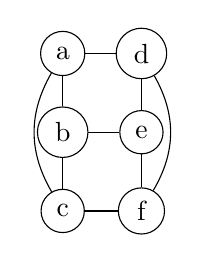
\begin{tikzpicture}[every node/.style={draw,circle}]
	\graph [simple] {
	a -- d;
	b -- e;
	c -- f;
	a -- b -- c --[bend left] a;
	d -- e -- f --[bend right] d;	
	}; 
\end{tikzpicture}
\end{center}

\section*{\texttt{3}}

\subsection*{(a)}

For any graph $G=(V,E)$, if we do a subdivision of $G$to obtain $G'$, we could
contract the added vertices and corresponding edges in order to recover $G$ from
$G'$. So, if $G$ holds a subgraph $G_{sub}$ isomorphic to a subdivision of $H$, denote
$H'$, we could delete all the vertices and edges which are not part of
$G_{sub}$, then we use the contraction on edges, edges deletion and vertices
deletion to obtain $H$.

\subsection*{(b)}

We use the following Petersen graph :

\begin{center}
\begin{tikzpicture}[every node/.style={draw,circle,very thick}]
  \graph [clockwise,math nodes] {
    subgraph C_n [V={a,b,c,d,e},name=A, radius=2cm]; 
    subgraph I_n [V={f,g,h,i,j},name=B, radius=1cm];
    \foreach \x [evaluate={%
        \i=alpha(\x);
        \j=alpha(mod(\x+1,5)+6); 
        \k=alpha(\x+5);}] in {1,...,5}{
      A \i -- B \k;
      B \j -- B \k;
    }
  }; 
\end{tikzpicture}    
\end{center}

The $K_5$ graph :

\begin{center}
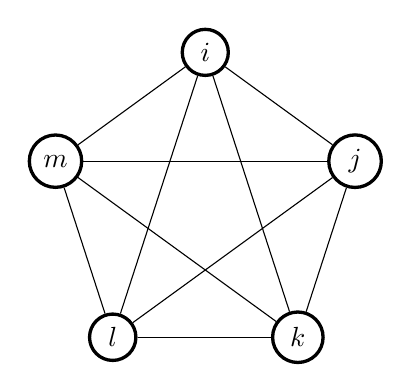
\begin{tikzpicture}[every node/.style={draw,circle,very thick}]
  \graph [clockwise,math nodes] {
    subgraph K_n [V={i,j,k,l,m},name=C,radius = 2cm]
  };
\end{tikzpicture}
\end{center}

The Petersen graph is not a subdivision of $K_{3,3}$, because the subdivision
could never delete edges. It only add a vertices $v$ on an edges $e =
\{v_1,v_2\}$ such that $E' = E \setminus \{v_1,v_2\} \cup
\{\{v_1,v\},\{v,v_2\}\}$ and $V' = V \cup \{v\}$.

So, we could never obtain the Petersen graph by successive subdivision because
we can't produce a vertices of degree $3$. We can't modifiy the degree of
existing vertices and the vertices obtained by subdivision are always of degrees
$2$.

The Petersen graph has $K_5$ has a minor. We use the following contraction in
order to obtain $k_5$ :
\begin{itemize}
\item \contract{a}{f}
\item \contract{b}{g}
\item \contract{c}{h}
\item \contract{d}{i}
\item \contract{e}{j}
\end{itemize}

\begin{center}
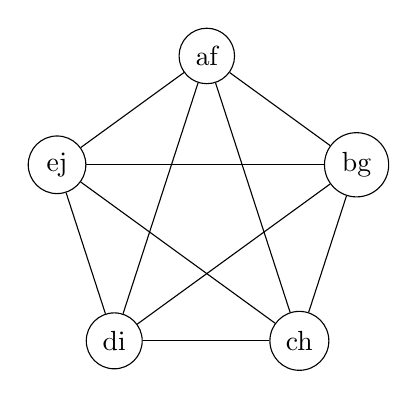
\begin{tikzpicture}[every node/.style={draw,circle}]
	\graph [simple,clockwise] {
		subgraph K_n [V={af,bg,ch,di,ej}, radius = 2cm];
	};
\end{tikzpicture}
\end{center}

\subsection*{(c)}

The subgraph $G'$, of the Petersen graph :

\begin{gather*}
  V = \{a,b,c,d,e,f,g,h,i,j\}\\
  E = \{
  \{a,f\},
  \{a,c\},
  \{a,b\},
  \{i,d\},
  \{d,e\},
  \{i,g\},
  \{g,b\},
  \{i,f\},
  \{h,f\},
  \{h,c\},
  \{c,b\},
  \{h,j\},
  \{j,e\},
  \}
\end{gather*}

We can ``see'' the subdivision of the $K_{3,3}$ graph, the blue nodes are from
the top groups, the red nodes are from the bottom groups and the gree nodes are
the from the subdivision of $K_{3,3}$.

\begin{center}
  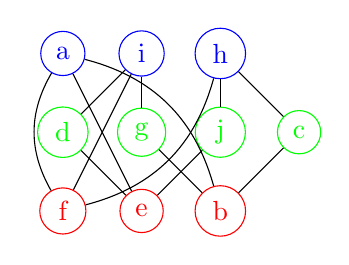
\begin{tikzpicture}[every node/.style={draw,circle}]
    \graph [simple, grow down, branch right] {
      {a[blue],i[blue],h[blue]} -!- {{},{d[green],g[green]},{j[green],c[green]}} -!- {{},{h[green]},{}} -!- {f[red],e[red],b[red]};
      a --[bend right] f;
      a -- e;
      a --[bend left] b;
      h -- {j -- e, c -- b};
      h --[bend left] f;
      i -- {f, d--e, g--b};
    };
  \end{tikzpicture}
\end{center}

is isomorphic to the following subdivision of $K_{3,3}$ :

The graph $K_{3,3}$ :

\begin{center}
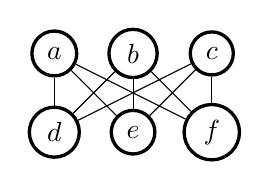
\begin{tikzpicture}[every node/.style={draw,circle,very thick}]
  \graph [branch right, grow down,math nodes] {
    subgraph K_nm [V={a,b,c},W={d,e,f}, radius=2cm]; 
  }; 
\end{tikzpicture}    
\end{center}

\section*{\texttt{4}}

\subsection*{(a)}

The bipartite graph we use :

\begin{center}
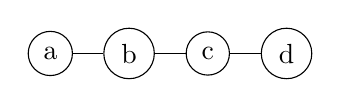
\begin{tikzpicture}[every node/.style={draw,circle}]
	\graph [simple] {
	a -- b -- c -- d;
	}; 
\end{tikzpicture}
\end{center}

Vertices ordering for the algorithm : $(a,d,b,c)$ :

\begin{enumerate}
\item Vertices $a$ : color $1$.
\item Vertices $d$ : color $1$.
\item Vertices $b$ : color $2$.
\item Vertices $c$ : color $3$.
\end{enumerate}

\subsection*{(b)}

For this, we use a Crown graph on $200$ vertices, the Crown graph is the
complete bipartite graph from which the edges of a perfect mathching has been
removed, for example, in the following $K_{4,4}$ graph :

\begin{center}
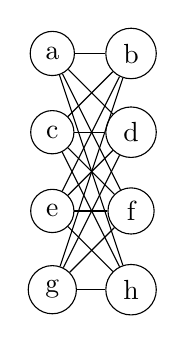
\begin{tikzpicture}[every node/.style={draw,circle}]
	\graph [simple] {
	subgraph K_nm [V={a,c,e,g},W={b,d,f,h}];
	}; 
\end{tikzpicture}
\end{center}

We have to remove the edges $\{a,b\},\{c,d\},\{e,f\},\{g,h\}$ (the edges from
vertices at the same height) to obtain a crown graph. Then we use the ordering
$(a,b,c,d,e,f,\cdots)$ (in alphabetical order) so, on $200$ vertices, the
chromatic number of the graph would be $100$.

\subsection*{(c)}

The following graph is bipartite and $5$-coloring

\begin{center}
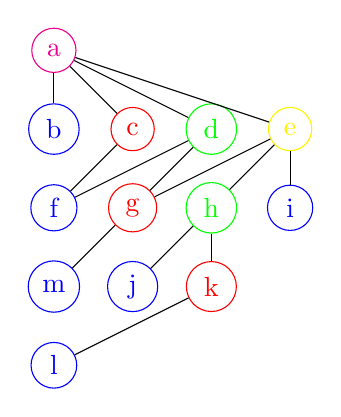
\begin{tikzpicture}[every node/.style={draw,circle}]
	\graph [simple, branch right, grow down] {
	{a[magenta]} -!- {b[blue],c[red],d[green],e[yellow]} -!- {f[blue],g[red],h[green],i[blue]}  -!- {m[blue],j[blue],k[red]} -!- {l[blue]};
	a -- {b,c,d,e};
	f -- {c,d};
	g -- {d,e};
	e -- {h,i};
	h -- {j,k};
	k -- l;
	m -- g;
	}; 
\end{tikzpicture}
\end{center}

under the ordering $(b,f,m,j,l,i,k,g,c,d,h,e,a)$.

\section*{\texttt{5}}

\subsection*{(a)}

We consider only the graph which has $1$ interior vertex, because the property
need to holds for every interior vertex, we can generalise this for any number
of interior vertex. We also consider $n$ exterior vertices $\{v_0,\cdots,v_n\}$
which are adjacent to the interior vertex $v$. The $n$ exterior vertices are
adjacent and it would be $2$ cases :
\begin{itemize}
\item $n$ is even : we have the subgraph $G' = (V',E')$ where $V' = V
  \setminus v$ and $E' = \{e  | e=\{x,y\} \in E \wedge (x \neq v \wedge y \neq
  v)\}$. $G'$ is $2$-coloring, so $G$ is $3$-coloring because $v$ is adjacent to
  vertices with color number $1$ and $2$ and $n$ is even.
\item $n$ is odd : we have the subgraph $G' = (V',E')$ where $V' = V
  \setminus v$ and $E\prime = \{e  | e=\{x,y\} \in E \wedge (x \neq v \wedge y \neq
  v)\}$. $G'$ is $3$-coloring, so $G$ is $4$-coloring and $n$ is odd.
\end{itemize}

So we avec to show that $C_n$ is $2$-coloring for $n$ even and $3$-coloring for
$n$ odd and $n \geq 3$. If $n$ is even, the graph is bipartite so $2$-coloring.
If $n$ is odd, we show that $C_n$ is $3$-coloring because we use $C_{n-1}$ and
we add a vertex between two already present one. We can only add a vertex
between vertices of color $1$ and $2$, so $C_n$ is $3$-coloring if $n$ is odd.

\subsection*{(b)}

From previous exercice, if $v$ has an odd number of adjacent vertices, it means
that the $C_n$ graph that is representing thos adjacent vertices is $3$-coloring
(or $2$-coloring if $deg(v) \equiv 0 \mod 2$). So if $deg(v)$ is even, $G$ is $3$-coloring.

\end{document}